\documentclass[lang=cn,10pt,newtx,color=green,thmcnt=section]{elegantbook}

% 封面信息
\title{《数学分析中的典型问题与方法》详解}
\subtitle{解析与扩充}
\author{李辉}
\date{2022年12月30日}
\bioinfo{学校}{南昌大学}
\extrainfo{由ElegantBook-4.4模板编写而成}

\setcounter{tocdepth}{3}
\logo{../image/logo-blue.png}
\cover{../image/cover.jpg}

% 本文档命令
\usepackage{array}
\newcommand{\ccr}[1]{\makecell{{\color{#1}\rule{1cm}{1cm}}}}

% 修改标题页的橙色带
\definecolor{customcolor}{RGB}{32,178,170}
\colorlet{coverlinecolor}{customcolor}
\usepackage{cprotect}

% 参考文献
\addbibresource[location=local]{reference.bib} 

% 双图
\usepackage{subfig}
\usepackage{graphicx}

% 长横箭头上写字
\usepackage{extarrows}

% 公式按节编号
\usepackage{amsmath}
\numberwithin{equation}{section}

% 公式编号
\usepackage{cleveref}
\crefname{equation}{式}{式}
\crefname{exam}{例题}{例题}
\crefname{exer}{练习}{练习}
\crefname{practice}{小试牛刀}{小试牛刀}

% 特殊符号
\usepackage{pifont}

% 浮动体
\usepackage{float}

\begin{document}

\maketitle
\frontmatter

\tableofcontents

\mainmatter

\chapter{一元函数极限}
\section{预备}
\subsection{几点注释}
\subsubsection{关于反函数}

\begin{definition}[反函数]
    给定集合$X$、$Y$,已知函数$f:X\rightarrow Y$,若函数$g$的定义域为$f(X)$,且
    \begin{equation*}
        \forall x\in X,有g(f(x))=x
    \end{equation*}
    即复合函数
    \begin{equation*}
        g\circ f:X\rightarrow f(X) \rightarrow X
    \end{equation*}是$X$上的恒等变换,则称$g$为$f$的反函数,且记$g=f^{-1}$
\end{definition}

\begin{note}
    \begin{itemize}
        \item $f$也是$f^{-1}$的反函数,即$(f^{-1})^{-1}=f$
        \item $f(f^{-1}(y))=y \quad f^{-1}(f(x))=x$\label{反函数性质}
    \end{itemize}
\end{note}

\begin{definition}[单射]
    已知函数$f:X\rightarrow Y$,若$\forall x_1,x_2 \in X$,
    \begin{equation*}
        x_1\ne x_2\Longrightarrow f(x_1)\ne f(x_2)
    \end{equation*}
    则称$f$为单射
\end{definition}

\begin{definition}[满射]
    已知函数$f:X\rightarrow Y$,若$\forall y \in Y$,
    \begin{equation*}
        \exists x \in X , f(x)=y
    \end{equation*}
    则称$f$为满射
\end{definition}

\begin{definition}[双射]
    已知函数$f:X\rightarrow Y$,若$f$既是单射,又是满射,则称$f$为双射。此时有
    \begin{equation*}
        \forall x_1 \ne x_2\in X \Longleftrightarrow f(x_1) \ne f(x_2)
    \end{equation*}
\end{definition}

\begin{theorem}[反函数存在的充分必要条件]
    函数$f$的反函数存在$\Longleftrightarrow$ $f$是双射
\end{theorem}

\begin{note}
    \begin{itemize}
        \item 若$f:X \rightarrow Y$和$g:Y\rightarrow Z$都是双射,则它们的复合函数$g\circ f$也是双射,且有
              \begin{equation*}
                  (g\circ f)^{-1}=f^{-1}\circ g^{-1}
              \end{equation*}

        \item 严格单调的满射必有反函数,且反函数与原函数保持相同的单调性
    \end{itemize}
\end{note}

\newpage

\begin{example}
    设$f:\mathbb{R} \rightarrow \mathbb{R}$严格单调增,$f^{-1}$是其反函数,$x_1$是$f(x)+x=a$的根,$x_2$是$f^{-1}(x)+x=a$的根,试求$x_1+x_2$的值.
\end{example}

\begin{solution}

    将$x_1$,$x_2$分别代入,得到
    \begin{equation}
        f(x_1)+x_1=a \label{x1方程}
    \end{equation}
    \begin{equation}
        f^{-1}(x_2)+x_2=a \label{x2方程}
    \end{equation}

    又由\ref{反函数性质}处的笔记可得,
    \begin{equation}
        x_1=f^{-1}(f(x_1)) \label{x1性质}
    \end{equation}

    将\cref{x1性质}代入\cref{x1方程}中,得到
    \begin{equation}
        f^{-1}(f(x_1))+f(x_1)=a \label{x1结果}
    \end{equation}

    对比\cref{x1结果}与\cref{x2方程},

    由于$f(x)$单调递增,则$f^{-1}(x)$也单调递增,进一步,$f^{-1}(x)+x$单调递增,最多只有一根,

    故$x_2=f(x_1)$

    即$x_1+x_2=x_1+f(x_1)=a$
\end{solution}

\subsubsection{关于函数奇偶性}

\begin{definition}[函数奇偶性]
    函数$f$定义在区间$(-l,l)$上($l$为正有限数或$+\infty$),

    若$\forall x\in (-l,l)$,有$f(x)=f(-x)$,则称函数$f$为偶函数。

    若$\forall x\in (-l,l)$,有$f(x)+f(-x)=0$,则称函数$f$为奇函数。
\end{definition}

\begin{example}
    设$f$是$(-l,l)$上的奇函数,并且有反函数$f^{-1}$,证明:$f^{-1}(x)$也是奇函数
\end{example}

\begin{proof}

    因为$f$是$(-l,l)$上的奇函数,所以$\forall x\in (-l,l)$,有
    \begin{equation}
        f(x)+f(-x)=0  \label{奇函数性质}
    \end{equation}

    $\forall y \in R_f=\{y|y=f(x) ,x\in (-l,l) \}$,有
    \begin{equation}
        f^{-1}(y)+f^{-1}(-y)=f^{-1}(f(x))+f^{-1}(-f(x))  \label{y替换为f(x)}
    \end{equation}

    将\cref{奇函数性质}代入\cref{y替换为f(x)},并由\ref{反函数性质}处笔记得到
    \begin{equation*}
        f^{-1}(y)+f^{-1}(-y)==f^{-1}(f(x))+f^{-1}(f(-x))=x+(-x)=0
    \end{equation*}

    即$f^{-1}(y)$在$R_f$上为奇函数
\end{proof}

\begin{example}
    若$f^{-1}$为$f$的反函数,$y=f^{-1}(-x)$是$y=f(-x)$的反函数,证明:$f$是奇函数
\end{example}

\begin{proof}

    由$f^{-1}$为$f$的反函数可得,
    \begin{equation}
        f(f^{-1}(y))=y \label{正逆函数}
    \end{equation}

    由$y=f^{-1}(-x)$是$y=f(-x)$的反函数可得,
    \begin{equation}
        f^{-1}(-f(-x))=x    \label{题目条件}
    \end{equation}

    结合\cref{正逆函数}、\cref{题目条件},
    \begin{equation*}
        f(x)+f(-x)=f(f^{-1}(-f(-x)))+f(-x)=-f(-x)+f(-x)=0
    \end{equation*}

    即$f$是奇函数
\end{proof}


\begin{example}
    证明:任一对称区间$(-l,l)$上的任一函数$f(x)$,总可以表示成一个奇函数$G(x)$与一个偶函数$H(x)$的和,而且此种表示方法是唯一的.
\end{example}

\begin{proof}

    假设已经找到一个奇函数$G(x)$与一个偶函数$H(x)$,使得
    \begin{equation}
        f(x)=G(x)+H(x) \label{式1}
    \end{equation}

    则由奇偶函数的性质可得,

    \begin{equation}
        f(-x)=G(-x)+H(-x)=-G(x)+H(x)    \label{式2}
    \end{equation}

    联立\cref{式1}、\cref{式2},

    可解得

    \begin{equation}
        G(x) = \frac{f(x)-f(-x)}{2} \label{奇函数决定式}
    \end{equation}
    \begin{equation}
        H(x) = \frac{f(x)+f(-x)}{2} \label{偶函数决定式}
    \end{equation}

    可由$f(x)$唯一确定\cref{奇函数决定式}、\cref{偶函数决定式},显然证毕
\end{proof}

\subsubsection{关于周期函数}
\begin{definition}[周期函数]
    若存在实数$T\ne 0$,使得$\forall x \in \mathbb{R} $,有
    \begin{equation*}
        f(x+T)=f(x)
    \end{equation*}

    则称函数$f$为以$T$为周期的周期函数
\end{definition}

\begin{note}
    \begin{itemize}
        \item 若$T$为函数$f$的周期,则其整数倍$kT$也为函数$f$的周期
        \item 若$T_1,T_2$均为函数$f$的周期,则$T_1\pm T_2$也为函数$f$的周期
        \item 并不是所有周期函数都有最小正周期, 如常值函数和狄利克雷 (Dirichlet)函数
    \end{itemize}
\end{note}

\begin{example}
    证明:设$f(x)$是$\mathbb{R}$上的有界实值函数,且有
    \begin{equation}
        f(x+h)=\frac{f(x+2h)+f(x)}{2} \quad (\forall x\in \mathbb{R})   \label{周期中间式}
    \end{equation}

    其中$h$为某一正数,则$h$必是函数$f$的周期
\end{example}

\begin{proof}

    整理\cref{周期中间式}得,
    \begin{equation}
        f(x+2h)-f(x+h)=f(x+h)-f(x)\quad(\forall x\in \mathbb{R})    \label{递推式1}
    \end{equation}

    令$F(x)=f(x+h)-f(x)$,则\cref{递推式1}化为
    \begin{equation}
        F(x+h)=F(x)
    \end{equation}

    则可得

    $f(x+nh)=[f(x+nh)-f(x+(n-1)h)]+[f(x+(n-1)h)-f(x+(n-2)h)]+\cdots+[f(x+h)-f(x)]+f(x)$
    $$=F(x+(n-1)h)+F(x+(n-2)h)+\cdots+F(x)+f(x)$$
    \begin{equation*}
        =\sum_{k=0}^{n-1}F(x+kh)+f(x)=nF(x)+f(x)
    \end{equation*}

    若$F(x)\ne 0$,则当$n\to +\infty$时,有$nF(x)\to \infty$

    则$f(x+nh)=nF(x)+f(x)\to \infty$,这与函数$f$有界矛盾,故$F(x)=0$

    即$f(x+h)=f(x)$,$h$为函数$f$的周期
\end{proof}

\begin{note}
    \begin{itemize}
        \item 若函数$f$在数轴上是有界函数,则\cref{周期中间式}或\cref{递推式1}是$f$以$h$为周期的充分必要条件
        \item “有界”条件必不可少,如$f(x)=x$
    \end{itemize}
\end{note}

\begin{example}\label{exer:周期例题}
    设$T$是$f$的正周期,$y=f^{-1}(x)$是$f$在$(0,T)$部分的反函数.试求$f$在$(-T,0)$部分的反函数.
\end{example}

\begin{solution}   \label{周期证明}

    $y=f^{-1}(x)$是$f$在$(0,T)$部分的反函数,则
    \begin{equation}
        f^{-1}(f(x))=x,\forall x \in (0,T) \label{周期性质}
    \end{equation}

    当$x \in (-T,0)$时,有$x+T\in (0,T)$,代入\cref{周期性质},得
    \begin{equation}
        f^{-1}(f(x+T))=x+T  \label{周期替换}
    \end{equation}

    又$f(x)$以$T$为周期,有
    \begin{equation}
        f(x+T)=f(x)
    \end{equation}

    代入\cref{周期替换},
    \begin{equation*}
        f^{-1}(f(x))=x+T
    \end{equation*}

    即
    \begin{equation*}
        f^{-1}(f(x))-T=x,\forall x \in (-T,0)
    \end{equation*}

    易知,$g(y)=f^{-1}(y)-T$为$f$在$(-T,0)$部分的反函数

\end{solution}

\begin{theorem}[反函数周期偏移]
    设函数$f$有正周期$T$,值域为$G=\{y|y=f(x),x \in \mathbb{R}\}$,$f^{-1}(y)$为其在$[0,T)$上的反函数,

    若$m\in [kT,(k+1)T)$,$k$为某整数,则在$[m,m+T)$上,

    $f$也有反函数,且该反函数由
    \begin{equation}
        x = \begin{cases}
            f^{-1}(y)+kT     & y\in \{y|y=f(x),x\in [m,(k+1)T)\}\subset G   \\
            f^{-1}(y)+(k+1)T & y\in \{y|y=f(x),x\in [(k+1)T,m+T)\}\subset G
        \end{cases}
    \end{equation}
\end{theorem}

\begin{proof}

    参见\cref{exer:周期例题}
\end{proof}

\subsection{几个常用的不等式}

\begin{theorem}[均值不等式]
    调和平均$\le$几何平均$\le$算术平均$\le$平方平均

    即

    $\forall x_i\ge 0(i=1,2,\cdots,n)$,恒有

    \begin{equation}    \label{均值不等式}
        \frac{n}{\frac{1}{x_1}+\cdots+\frac{1}{x_n}}\le \sqrt[n]{x_1\cdots x_n}\le  \frac{x_1+\cdots+x_n}{n} \le \sqrt{\frac{x_1^2+\cdots+x_n^2}{n}}
    \end{equation}

    当且仅当$x_1=\cdots=x_n$时取等号
\end{theorem}

\begin{proof}

    [几何平均$\le$算术平均]

    \vspace{4pt}

    显然
    \begin{equation}
        \sqrt{x_1x_2}=\sqrt{(\frac{x_1+x_2}{2})^2-(\frac{x_1-x_2}{2})^2}\le \frac{x_1+x_2}{2}   \label{2}
    \end{equation}

    当且仅当$x_1=x_2$时取等号

    这说明$n=2$时,不等式成立
    \vspace{6pt}

    $n=4$时,由\cref{2}得,
    \begin{equation}
        \sqrt[4]{x_1x_2x_3x_4}=\sqrt{\sqrt{x_1x_2}\sqrt{x_3x_4}}\le \frac{\sqrt{x_1x_2}+\sqrt{x_3x_4}}{2}\le \frac{\frac{x_1+x_2}{2}+\frac{x_3+x_4}{2}}{2}=\frac{x_1+x_2+x_3+x_4}{4}    \label{4递推}
    \end{equation}

    当且仅当$x_1=x_2=x_3=x_4$时取等号

    这说明$n=4$时,不等式成立
    \vspace{8pt}

    假设$n=2^k$时,不等式成立,即
    \begin{equation}
        \sqrt[2^k]{x_1\cdots x_{2^k}}\le \frac{x_1+\cdots+x_{2^k}}{2^k}
    \end{equation}

    当且仅当$x_1=x_2=\cdots = x_{2^k}$时取等号

    \vspace{8pt}

    则$n=2^{k+1}$时,

    \begin{equation*}
        \sqrt[2^{k+1}]{x_1\cdots x_{2^k}\cdots x_{2^{k+1}}}=\sqrt[2^k]{\sqrt{x_1 x_2} \sqrt{x_3 x_4} \cdots \sqrt{x_{2^{k+1}-1} x_{2^{k+1}}}}\le \frac{\sqrt{x_1 x_2}+\sqrt{x_3 x_4}+\cdots+\sqrt{x_{2^{k+1}-1} x_{2^{k+1}}}}{2^k}
    \end{equation*}
    \begin{equation}
        \le \frac{ \frac{x_1+x_2}{2} + \frac{x_3+x_4}{2} + \cdots + \frac{x_{2^{k+1}-1}+x_{2^{k+1}}}{2}}{2^k} = \frac{x_1+x_2+\cdots + x_{2^{k+1}-1}+x_{2^{k+1}}}{2^{k+1}}=\frac{x_1+x_2+\cdots + x_{2^{k+1}-1}+x_{2^{k+1}}}{n}
    \end{equation}

    当且仅当$x_1=x_2=\cdots = x_{2^{k+1}}$时取等号

    \vspace{8pt}

    即,对$n=2^k(k=1,2,\cdots)$,不等式均成立

    \vspace{8pt}
    设$A=\frac{x_1+\cdots+x_n}{n}$,

    设对$n+1$,不等式成立,则
    \begin{equation}
        A=\frac{nA+A}{n+1}=\frac{x_1+\cdots+x_n+A}{n+1}\ge \sqrt[n+1]{x_1\cdots x_n A}
    \end{equation}

    整理得,

    \begin{equation}
        A^{n+1}\ge x_1\cdots x_n A \implies A\ge \sqrt[n]{x_1 \cdots x_n}
    \end{equation}

    即对$n$,不等式成立

    由数学归纳法,对$n=1,2,\cdots$,不等式均成立

    \vspace{8pt}

    [调和平均$\le$几何平均]

    \vspace{4pt}
    在“几何平均$\le$算术平均”不等式中,令$x_i=\frac{1}{a_i}(i=1,2\cdots)$,有

    \begin{equation}
        \sqrt[n]{\frac{1}{a_1}\cdots \frac{1}{a_n}} \le \frac{\frac{1}{a_1}+\cdots+\frac{1}{a_n}}{n}
    \end{equation}

    整理得,

    \begin{equation}
        \frac{n}{\frac{1}{a_1}+\cdots+\frac{1}{a_n}}\le \sqrt[n]{a_1\cdots a_n}
    \end{equation}

    得证

    \vspace{8pt}
    [算术平均$\le$平方平均]

    由柯西不等式得,
    \begin{equation*}
        (x_1+\cdots+x_n)^2=(x_1\cdot1 +\cdots +x_n\cdot1)^2\le (x_1^2+\cdots+x_n^2)(1+\cdots+1)=n(x_1^2+\cdots+x_n^2)
    \end{equation*}
    \begin{equation}
        (\frac{x_1+\cdots+x_n}{n})^2 \le \frac{x_1^2+\cdots +x_n^2}{n}
    \end{equation}

    两边开方即得证
\end{proof}

\vspace{8pt}

\begin{theorem}[对数不等式]\label{定理1.1.4}
    当$x>-1$时,有
    \begin{equation}
        \frac{x}{1+x} \le \ln(1+x) \le x
    \end{equation}

    当且仅当$x=0$时取等号
\end{theorem}

\begin{figure}[htbp]
    \centering
    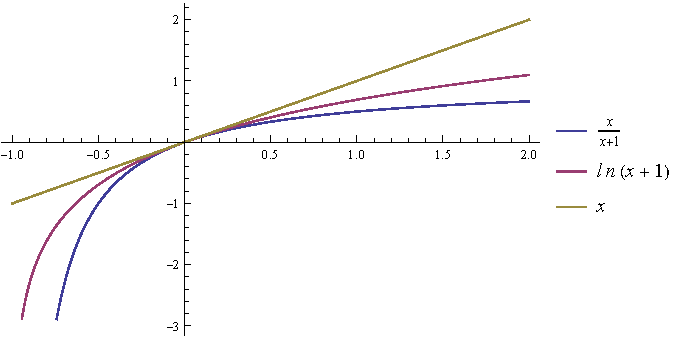
\includegraphics[width=0.8\textwidth]{../image/对数不等式.pdf}
    \caption{对数不等式图解}
\end{figure}

\begin{solution}
    求导证明即可
\end{solution}

\begin{note}
    \begin{itemize}
        \item 令$x=\frac{1}{n}$,则可以得到
              \begin{equation}
                  \frac{1}{1+n} \le \ln(1+\frac{1}{n}) \le \frac{1}{n} \label{对数不等式推论}
              \end{equation}
    \end{itemize}
\end{note}

\begin{figure}[htbp]
    \centering
    \subfloat
    {
        \begin{minipage}[t]{0.49\textwidth}
            \centering
            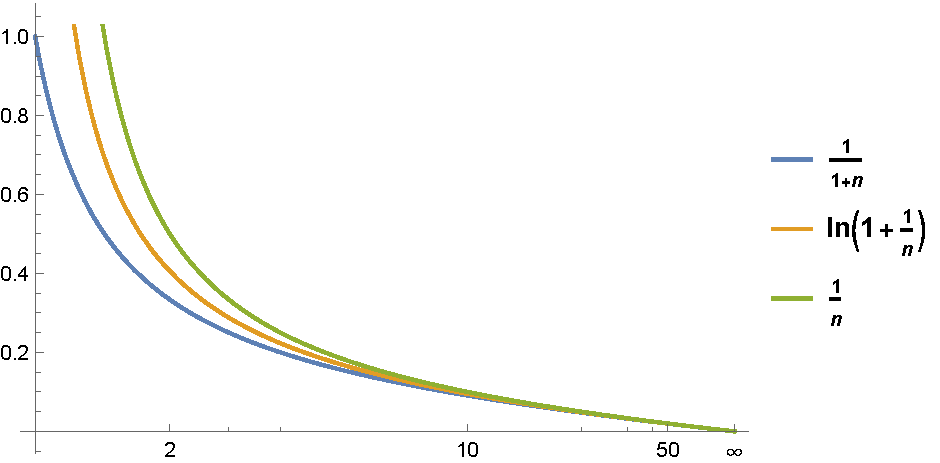
\includegraphics[width=\textwidth]{../image/对数不等式推论}
        \end{minipage}
    }
    \subfloat
    {
        \begin{minipage}[t]{0.49\textwidth}
            \centering
            \includegraphics[width=\textwidth]{../image/sinx与x}
        \end{minipage}
    }
    \vspace{6pt}
    \caption{不等式\ref{对数不等式推论}(左)、不等式\ref{1.37}(右)图解}
\end{figure}

\begin{example}
    证明:\begin{equation}
        \frac{2}{\pi}x \le \sin x \le x \quad x\in (0,\frac{\pi}{2}) \label{1.37}
    \end{equation}
\end{example}

\begin{proof}
    考虑$f(x)=\frac{\sin x}{x}$,求导证明即可
\end{proof}

\subsection{华里士(Wallis)公式}
\begin{theorem}[Wallis公式]
    \begin{equation}
        I_n=\int_{0}^{\frac{\pi}{2}} \sin^n xdx=\int_{0}^{\frac{\pi}{2}} \cos^n xdx=
        \begin{cases}
        \frac{(n-1)!!}{n!!} \cdot \frac{\pi}{2}& n=2k\\ 
        \frac{(n-1)!!}{n!!}& n=2k+1
        \end{cases}
    \end{equation}

    \begin{equation}
        I_{m,n}=\int_{0}^{\frac{\pi}{2}}\sin^m x \cos^n xdx=
    \begin{cases}
        \frac{(m-1)!!(n-1)!!}{(m+n)!!}\cdot \frac{\pi}{2} & m=2i,n=2j\\ 
        \frac{(m-1)!!(n-1)!!}{(m+n)!!}& others
    \end{cases}
    \end{equation}
\end{theorem}

\begin{proof}
    
    [$I_n$前部分]
    
    由分部积分法,
    \begin{equation*}
        I_n=\int_{0}^{\frac{\pi}{2}} \sin^n xdx
        =-\int_{0}^{\frac{\pi}{2}} \sin^{n-1}x d \cos x
        =-\sin^{n-1} x \cos x|_{0}^{\frac{\pi}{2}}+\int_{0}^{\frac{\pi}{2}} \cos x d \sin^{n-1} x
    \end{equation*}

    \begin{equation*}
        =\int_{0}^{\frac{\pi}{2}} \cos x\cdot (n-1)\sin^{n-2} x \cdot \cos x dx
        =(n-1)\int_{0}^{\frac{\pi}{2}} \cos^2 x \sin^{n-2} x dx
    \end{equation*}

    \begin{equation*}
        =(n-1)\int_{0}^{\frac{\pi}{2}} (1-\sin^2 x) \sin^{n-2} x dx
        =(n-1)\int_{0}^{\frac{\pi}{2}}\sin^{n-2} xdx - (n-1)\int_{0}^{\frac{\pi}{2}}\sin^n xdx
    \end{equation*}

    \begin{equation*}
        = (n-1)I_{n-2}-(n-1)I_n
    \end{equation*}

    整理得迭代式:

    \begin{equation}
        I_n = \frac{n-1}{n} I_{n-2} \label{点火迭代式}
    \end{equation}
    
    又
    \begin{equation*}
        I_0 = \int_{0}^{\frac{\pi}{2}} dx = \frac{\pi}{2}
    \end{equation*}
    \begin{equation*}
        I_1 = \int_{0}^{\frac{\pi}{2}} \sin x dx = -\cos x|_{0}^{\frac{\pi}{2}} = 1 
    \end{equation*}

    依据\cref{点火迭代式}迭代得,\
    \begin{equation}
        I_n = \frac{n-1}{n} I_{n-2}
        = \frac{n-1}{n} \frac{n-3}{n-2} I_{n-4}=\cdots 
        \begin{cases}
            = \frac{n-1}{n} \frac{n-3}{n-2} \cdots \frac{1}{2}I_0 = \frac{(n-1)!!}{n!!} \cdot \frac{\pi}{2}& n=2k\\
            = \frac{n-1}{n} \frac{n-3}{n-2} \cdots \frac{2}{3}I_1 = \frac{(n-1)!!}{n!!} & n=2k+1
        \end{cases}
    \end{equation}
    
    得证

    [$I_n$后部分]

    \begin{equation*}
        \int_{0}^{\frac{\pi}{2}} \cos^n xdx
        \xlongequal{t=\frac{\pi}{2}-x}
        \int_{\frac{\pi}{2}}^{0}\cos^n (\frac{\pi}{2}-t)d(\frac{\pi}{2}-t) = - \int_{\frac{\pi}{2}}^{0}\sin^n tdt
        = \int_{0}^{\frac{\pi}{2}} \sin^n tdt =I_n 
    \end{equation*}

    得证

    [$I_{m,n}$]

    \begin{equation*}
        I_{m,n} = \int_{0}^{\frac{\pi}{2}}\sin^m x \cos^n xdx
        = \int_{0}^{\frac{\pi}{2}}\sin^m x \cos^{n-1} xd \sin x
    \end{equation*}
    \begin{equation*}
        = \sin^{m+1} x \cos^{n-1} x |_{0}^{\frac{\pi}{2}}-
        \int_{0}^{\frac{\pi}{2}}\sin x d (\sin^m x \cos^{n-1}x) 
    \end{equation*}
    \begin{equation*}
        =-\int_{0}^{\frac{\pi}{2}}\sin x  (m\sin^{m-1}x \cos x \cos^{n-1}x - sin^m x (n-1)\cos^{n-2} x \sin x) dx
    \end{equation*}
    \begin{equation*}
        =-m\int_{0}^{\frac{\pi}{2}}\sin^m x \cos^{n}xdx +(n-1) \int_{0}^{\frac{\pi}{2}} sin^{m+2} x \cos^{n-2} x dx
        = -m I_{m,n}+(n-1)I_{m+2,n-2}
    \end{equation*}

    整理得,

    \begin{equation}
        I_{m,n} = \frac{n-1}{m+1} I_{m+2,n-2}   \label{迭代式2}
    \end{equation}

    \vspace{8pt}
    $\star \quad n=2k$时,依据迭代\cref{迭代式2},有
    \begin{equation*}
        I_{m,n}=\frac{n-1}{m+1} I_{m+2,n-2}
        = \frac{n-1}{m+1} \frac{n-3}{m+3} I_{m+4,n-4}
        = \frac{n-1}{m+1} \frac{n-3}{m+3}\cdots \frac{1}{m+n-1} I_{m+n}
        = \frac{(n-1)!!(m-1)!!}{(m+n-1)!!} I_{m+n}
    \end{equation*}
    \begin{equation}
        =
        \begin{cases}
            \frac{(n-1)!!(m-1)!!}{(m+n-1)!!} \frac{(m+n-1)!!}{(m+n)!!} \cdot \frac{\pi}{2}=\frac{(n-1)!!(m-1)!!}{(m+n)!!} \cdot \frac{\pi}{2}& m=2k\\
            \frac{(n-1)!!(m-1)!!}{(m+n-1)!!} \frac{(m+n-1)!!}{(m+n)!!} = \frac{(n-1)!!(m-1)!!}{(m+n)!!} & m=2k+1 \label{1.38}
        \end{cases}
    \end{equation}

    \vspace{8pt}
    $\star \quad n=2k+1$时,依据迭代\cref{迭代式2},有
    \begin{equation}
        I_{m,n}=\frac{n-1}{m+1} I_{m+2,n-2}
        = \frac{n-1}{m+1} \frac{n-3}{m+3} I_{m+4,n-4}
        = \frac{n-1}{m+1} \frac{n-3}{m+3}\cdots \frac{2}{m+n-2} I_{m+n-1,1}
        = \frac{(n-1)!!(m-1)!!}{(m+n-2)!!} I_{m+n-1,1}  \label{1.39}
    \end{equation}

    又有
    \begin{equation}
        I_{m+n-1,1} = \int_{0}^{\frac{\pi}{2}} \sin^{m+n-1} x \cos xdx
        = \int_{0}^{\frac{\pi}{2}} \sin^{m+n-1} x d\sin x
        = \frac{1}{m+n} \sin^{m+n} x|_{0}^{\frac{\pi}{2}}
        = \frac{1}{m+n} \label{1.40}
    \end{equation}

    将\cref{1.40}代入\cref{1.39}得,无论$m$的奇偶性,均有
    \begin{equation}
        I_{m,n} = \frac{(n-1)!!(m-1)!!}{(m+n)!!}    \label{1.41}
    \end{equation}

    结合\cref{1.38}、\cref{1.41},得证
\end{proof}

\subsection{练习}

\begin{exercise}
    求复合函数的表达式

    (1)已知$f(x)=\frac{x}{\sqrt{1+x^2}}$,设$f_n(x)=f\{f[\cdots (f(x)) \cdots]\}(n$个$f)$,求$f_n(x)$

    (2)设$f(x)=\frac{x}{x-1}$,试证明$f[f(f(x))]=f(x)$,并求$f(\frac{1}{f(x)})\quad (x\ne 0,x\ne 1)$
\end{exercise}

\begin{solution}

    (1)
    \begin{equation*}
        f_2(x)=\frac{\frac{x}{\sqrt{1+x^2}}}{\sqrt{1+(\frac{x}{\sqrt{1+x^2}})^2}} = \frac{x}{\sqrt{1 + 2 x^2}}
    \end{equation*}
    \begin{equation*}
        f_3(x)=\frac{\frac{x}{\sqrt{1+2x^2}}}{\sqrt{1+(\frac{x}{\sqrt{1+2x^2}})^2}} = \frac{x}{\sqrt{1 + 3 x^2}}
    \end{equation*}

    设$n=k$时,有$f_k(x)=\frac{x}{\sqrt{1 + k x^2}}$

    则$n=k+1$时,\begin{equation*}
        f_{k+1}(x)=\frac{\frac{x}{\sqrt{1+kx^2}}}{\sqrt{1+(\frac{x}{\sqrt{1+kx^2}})^2}} = \frac{x}{\sqrt{1 + (k+1) x^2}}
    \end{equation*}

    由数学归纳法得,$f_n(x)=\frac{x}{\sqrt{1 + n x^2}}$

    (2)

    \begin{equation*}
        f(f(x)) = \frac{\frac{x}{x-1}}{\frac{x}{x-1}-1} = \frac{x}{x-(x-1)} = x
    \end{equation*}
    \begin{equation*}
        f[f(f(x))] = \frac{x}{x-1} = f(x)
    \end{equation*}

    得证
    \begin{equation*}
        \frac{1}{f(x)} = \frac{x-1}{x}
    \end{equation*}
    \begin{equation*}
        f(\frac{1}{f(x)}) = \frac{\frac{x-1}{x}}{\frac{x-1}{x}-1} = \frac{x-1}{x-1-x} = 1-x
    \end{equation*}
\end{solution}

\begin{exercise}
    是否存在这样的函数,它在区间[0,1]上每点取有限值,在此区间上的任何点的任意领域内无界.
\end{exercise}

\begin{solution}
    
    存在。如:
    \begin{equation}
        f(x) = 
        \begin{cases}
            n & x=\frac{m}{n},m\mbox{、}n\mbox{互质},n>0\\ 
            0 & x\mbox{为无理数}
        \end{cases}
    \end{equation}

    \begin{figure}[htbp]
        \centering
        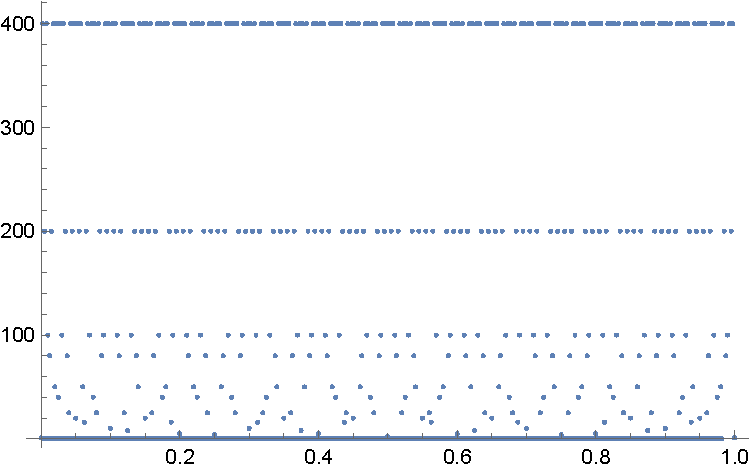
\includegraphics[width=0.6\textwidth]{../image/狄利克雷函数}
        \caption{在区间[0,1]上每点取有限值\\ 在此区间上的任何点的任意领域内无界}
    \end{figure}
\end{solution}

\begin{exercise}
    试说明能有无穷多个函数,其中每个函数$f$,均能使得$f\circ f$为$R$上的恒等函数。
\end{exercise}

\begin{solution}
    $f\circ f$为$R$上的恒等函数$\Longrightarrow $ $f$为自己的反函数

    事实上,给定任意函数$g:(0,+\infty) \to (-\infty,0)$

    以$g(x)\mbox{和}g^{-1}(x)$构造以下的函数$f$:
    \begin{equation*}
        f(x)
        = \begin{cases}
            g(x) & x\in (0,+\infty)\\ 
            0 & x=0 \\ 
            g^{-1}(x) & x \in (-\infty,0)
        \end{cases}
    \end{equation*}

    $f\circ f$即为恒等函数
\end{solution}

\begin{exercise}
    设$f$为$R$上的奇函数,$f(1)=a$,$f(x+2)-f(x)=f(2),\forall x \in \mathbb{R}$ .

    (1)试用$a$表达$f(2)$和$f(5)$

    (2)$\ a$为何值时,$f(x)$是以2为周期的周期函数. 
\end{exercise}

\begin{solution}
    
    (1)
    当$x=-1$时,有
    \begin{equation*}
        f(1)-f(-1) = 2f(1) = f(2)
    \end{equation*}

    则$f(2)=2a$

    当$x=1$时,有
    \begin{equation*}
        f(3)-f(1) = f(2)
    \end{equation*}

    则$f(3)=f(1)+f(2)=3a$

    当$x=3$时,有
    \begin{equation*}
        f(5)-f(3) = f(2)
    \end{equation*}

    则$f(5)=f(3)+f(2)=5a$

    (2)若$f(x)$是以2为周期的周期函数,则有
    \begin{equation*}
        f(x+2)-f(x)=0=f(2)
    \end{equation*}

    故 $f(2)=2a=0 \Rightarrow a=0$
\end{solution}

\begin{exercise}
    设$f(x)=1-x+\lfloor x \rfloor$,$g(x)=\sec x$,说明这时$f(x)-g(x)$为什么不是周期函数.类似地,$f(x)+g(x)$也如此.从而周期函数的和和差未必是周期函数.
\end{exercise}

\begin{solution}
    
    易得,$f(x)$以$T_1=1$为最小正周期,$g(x)$以$T_2=2\pi$为周期

    假设$f(x)-g(x)$以$T$为周期,则有
    \begin{equation*}
        f(x+T)-g(x+T)=f(x)-g(x)
    \end{equation*}

    令$x=0$,有
    \begin{equation*}
        f(T)-g(T)=f(0)-g(0)=0
    \end{equation*}
    
    即
    \begin{equation}
        1-T+\lfloor T \rfloor= \sec T   \label{1.1.43}
    \end{equation}

    \cref{1.1.43}仅在$T=0$时成立,这与周期不等于0矛盾

    故$f(x)-g(x)$不是周期函数

    同理得,$f(x)+g(x)$也不是周期函数
\end{solution}

\begin{figure}[H]
    \centering
    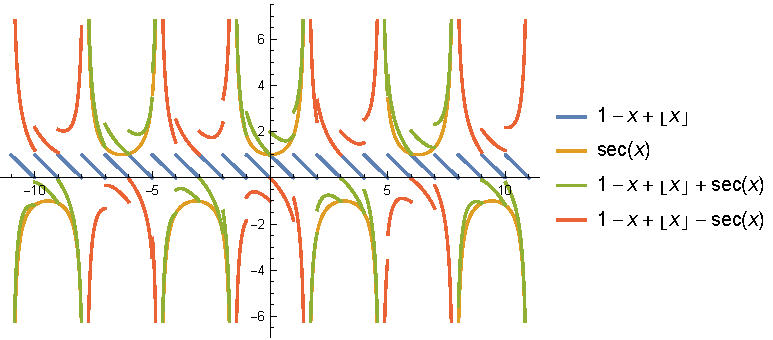
\includegraphics[width=0.7\textwidth]{../image/1-x+[x]}
    \caption{周期函数之和差未必为周期函数}
\end{figure}

\begin{exercise}[$\ $(双镜效应)]
    设$f$是$\mathbb{R}$上的实值函数,$f$的图像以直线$x=b$和直线$x=c(b\ne c)$为对称轴,试证$f$必是周期函数,且周期为$T=2|b-c|$
\end{exercise}

\begin{proof}
    
    $f$的图像以直线$x=b$和直线$x=c(b\ne c)$为对称轴,则有
    \begin{equation}
        f(x)=f(2b-x) \label{1.1.44}
    \end{equation}
    \begin{equation}
        f(x)=f(2c-x)    \label{1.1.45}
    \end{equation}
    
    联立\cref{1.1.44},\cref{1.1.45},得
    \begin{equation*}
        f(2b-x)=f(2c-x)
    \end{equation*}

    令$t=2b-x$,则$x=2b-t$
    \begin{equation*}
        f(t)=f(t+2c-2b)
    \end{equation*}

    即$f$是周期函数,且以$T=2|b-c|$为周期
\end{proof}

\begin{exercise}
    设$f$是$\mathbb{R}$上的奇函数,并且以直线$x=a(a\ne 0)$作为对称轴,试证$f$必为周期函数,并求其周期. 
\end{exercise}

\begin{proof}

    $f$是$\mathbb{R}$上的奇函数,则
    \begin{equation}
        f(x)=-f(-x) \label{1.1.46}
    \end{equation}

    $f$以直线$x=a(a\ne 0)$作为对称轴,则
    \begin{equation}
        f(x)=f(2a-x)    \label{1.1.47}
    \end{equation}

    多次利用\cref{1.1.46},\cref{1.1.47},得
    \begin{equation*}
        f(x)=f(2a-x)=-f(x-2a)=-f(2a-(x-2a))=-f(4a-x)=f(x-4a)
    \end{equation*}
    
    故$f$为周期函数,周期为$T=4|a|$. 
\end{proof}

\vspace{5pt}
\begin{exercise}
    设$f$为$\mathbb{R}$上以$T$为周期的周期函数$(T>0)$,且$f$在$[0,T)$上严格单调增,试证明$f(x^2)$不可能是周期函数. 
\end{exercise}

\begin{proof}

    假设$f(x^2)$以$T_0(T_0\ne 0)$为周期,则有
    \begin{equation}
        f((x+T_0)^2)=f(x^2+2xT_0+T_0^2)=f(x^2)  \label{1.1.48}
    \end{equation}

    令$x=0$,则
    \begin{equation*}
        f(T_0^2)=f(0)
    \end{equation*}

    又$f$在$[0,T)$上严格单调增,

    故$f(x)$在一个周期内不肯能相等,则
    \begin{equation}
        T_0^2=nT \quad \mbox{n为正整数} \label{1.1.49}
    \end{equation}

    将\cref{1.1.49}代入\cref{1.1.48},得
    \begin{equation*}
        f(x^2+2x\sqrt{nT}+nT)=f(x^2)
    \end{equation*}

    令$x=\sqrt{(n+1)T}$,
    \begin{equation*}
        f((n+1)T+2\sqrt{n(n+1)}T+nT)=f((n+1)T)
    \end{equation*}
    \begin{equation*}
        f(2\sqrt{n(n+1)}T)=f(0)\Longrightarrow \sqrt{n(n+1)}\mbox{为正整数}
    \end{equation*}

    但相邻两正整数之乘积不可能是平方数, 产生矛盾

    故$f(x^2)$不可能是周期函数
\end{proof}

\begin{exercise}
    证明确界的关系式:

    (1)叙述数集$A$的确界定义,并证明:
    对于任意有界数列$\{x_n\}$,$\{y_n\}$,总有
    \begin{equation}
        \sup\{x_n+y_n\}\le \sup\{x_n\}+\sup\{y_n\}
    \end{equation}

    (2)设$A,B$是两个由非负数组成的任意数集,试证明:
    \begin{equation}
        \underset{x\in A}{\sup x} \cdot \underset{y \in B}{\sup y} = \underset{y \in B}{\underset{x \in A}{\sup xy}}
    \end{equation}
\end{exercise}

\begin{proof}
    (1)确界定义:
    
    设非空数集A有上界,若存在实数$\beta$满足以下两个条件:

    \ding{172}$\forall x\in A$,有$x\le \beta$\quad($\beta$是$A$的上界)
    \qquad
    \ding{173}$\forall \epsilon>0$,$\exists x_0 \in A$,有$x_0>\beta - \epsilon$ \quad ($\beta$是$A$的最小上界)

    则称$\beta$为$A$的上确界,记为$\sup A$
    \vspace{3pt}

    设非空数集A有下界,若存在实数$\alpha$满足以下两个条件:

    \ding{172}$\forall x\in A$,有$x\ge \alpha$\quad($\alpha$是$A$的下界)
    \qquad
    \ding{173}$\forall \epsilon>0$,$\exists x_0 \in A$,有$x_0<\alpha + \epsilon$ \quad ($\alpha$是$A$的最大下界)

    则称$\alpha$为$A$的下确界,记为$\inf A$

    \vspace{3pt}
    $\forall n$,$x_n+y_n\le \sup\{x_n\}+\sup\{y_n\}$,
    故$\sup\{x_n\}+\sup\{y_n\}$为$\{x_n+y_n\}$的一个上界

    由上确界的定义得,$\sup\{x_n+y_n\}\le \sup\{x_n\}+\sup\{y_n\}$

    \vspace{3pt}
    (2)一方面,有$0\le x \le \underset{x\in A}{\sup x}(\forall x\in A)$,
    $0 \le y \le \underset{y\in B}{\sup y}(\forall y\in B)$,
    可得$0\le xy \le \underset{x\in A}{\sup x}\cdot \underset{y\in B}{\sup y} (\forall x\in A,\forall y\in B)$

    故$\underset{x\in A}{\sup x}\cdot \underset{y\in B}{\sup y} $是$\{xy|\forall x\in A,\forall y\in B\}$的一个上界,
    由上确界的定义得,$\underset{y \in B}{\underset{x \in A}{\sup xy}}\le \underset{x\in A}{\sup x}\cdot \underset{y\in B}{\sup y}$

    另一方面,$\forall x\in A$,有$xy \le \underset{y \in B}{\underset{x \in A}{\sup xy}}(\forall y \in B)$,故$\underset{y \in B}{\underset{x \in A}{\sup xy}}(\forall y \in B)$为$\{xy|\forall y \in B\}$的一个上界,

    由上确界的定义得,$x \cdot \underset{y\in B}{\sup y} \le \underset{y \in B}{\underset{x \in A}{\sup xy}}(\forall x\in A)$

    故$\underset{y \in B}{\underset{x \in A}{\sup xy}}$为$\{x \cdot \underset{y\in B}{\sup y}|\forall x\in A\}$的一个上界,由上确界的定义得,$\underset{x\in A}{\sup x} \cdot \underset{y \in B}{\sup y} \le \underset{y \in B}{\underset{x \in A}{\sup xy}}$

    综上,$\underset{x\in A}{\sup x} \cdot \underset{y \in B}{\sup y} = \underset{y \in B}{\underset{x \in A}{\sup xy}}$
\end{proof}

\begin{exercise}
    试证明:若$\underset{n \to \infty}{\lim}x_n=+\infty$,则$\{x_n\}$必达到下确界(即$\exists m \in \mathbb{N}$,使得$x_m=\inf \{x_n\}$). 
\end{exercise} 

\begin{proof}
    $\underset{n \to \infty}{\lim}x_n=+\infty$,
    故$\forall M,\exists N \in \mathbb{N^+}$,使得$\forall n>N$时,有$x_n>M$,

    令$M=x_1$,则$\exists N \in \mathbb{N^+}$,使得$\forall n>N$时,有$x_n>x_1$,

    取$x_m=\min \{x_1,x_2,\cdots,x_N\}$,

    则$\forall n \in \mathbb{N^+}$,$x_n\ge x_m$,又$x_m \in \{x_n\}$,则$x_m=\inf \{x_n\}$
\end{proof}

\begin{exercise}
    设$f,g$是$\mathbb{R}$上的实值函数,且
    \begin{equation*}
        f(x+y)+f(x-y)=2f(x)g(y)\quad \forall x,y\in \mathbb{R}
    \end{equation*}

    在$\mathbb{R}$上,$f(x)$不恒等于0,但有界,试证明:$|g(y)|\le 1 (\forall y \in \mathbb{R})$
\end{exercise}

\begin{proof}
    $f(x)$有界$\Longrightarrow |f(x)|$有界 

    由确界原理得,$|f(x)|$有上确界$M$,即$\forall \epsilon >0,\exists x\in \mathbb{R},$使得$M-\epsilon<|f(x)|\le M$

    对此处的$\epsilon$和$x$,有$\forall y\in \mathbb{R}$
    \begin{equation*}
        2M\ge |f(x+y)|+|f(x-y)|\ge |f(x+y)+f(x-y)|=|2f(x)g(y)|
    \end{equation*}
    \begin{equation*}
        =2|f(x)||g(y)|>2(M-\epsilon)|g(y)|
    \end{equation*}

    令$\epsilon \to 0$,则有
    \begin{equation*}
        2M \ge 2M |g(y)|
    \end{equation*}

    即$|g(y)|\le 1$,得证
\end{proof}

\begin{exercise}
    设$f$是闭区间$[a,b]$上的增函数(不一定连续),如果$f(a)\ge a$,$f(b)\le b$,试证明:$\exists x_0 \in [a,b]$,使得$f(x_0)=x_0$
\end{exercise}

\begin{proof}
    
    $f(a)\ge a \Longrightarrow A=\{x|f(x)\ge x\}\subset [a,b]$非空有界$\xlongrightarrow{\mbox{确界原理}}$ $x_0=\sup A\in [a,b]$有意义

    \ding{172}若$y_0=f(x_0)>x_0$,由于$f$单调增,有$f(y_0)\ge f(x_0)=y_0$,则$y_0\in A$
    
    故$y_0\le \sup A=x_0$,产生矛盾

    \ding{173}若$y_0=f(x_0)<x_0$,由$x_0=\sup A$得,$\exists x_1\in A$,有$y_0<x_1<x_0$,

    由$f$单调增及$x_1 \in A$,可得$f(x_1)\le f(x_0)=y_0<x_1\le f(x_1)$

    即$f(x_1)<f(x_1)$,产生矛盾

    综上所述,$y_0=f(x_0)=x_0$
\end{proof}

\begin{exercise}
    设$f(x)$在$[0,1]$上单调增,$f(0)>0$,$f(1)<1$. 
    试证明:$\exists x_0 \in (0,1)$,使得$f(x_0)=x_0^2$
\end{exercise}

\begin{proof}

    $f(0)> 0 \Longrightarrow A=\{x|f(x)\ge x^2\}\subset [0,1]$非空有界$\xlongrightarrow{\mbox{确界原理}}$ $x_0=\sup A\in [0,1]$有意义

    \ding{172}若$y_0=f(x_0)>x_0^2$,则$\sqrt{y_0}>x_0,$由于$f$单调增,有$f(\sqrt{y_0})> f(x_0)=y_0=(\sqrt{y_0})^2$,则$\sqrt{y_0}\in A$
    
    故$\sqrt{y_0}\le \sup A=x_0$,产生矛盾

    \ding{173}若$y_0=f(x_0)<x_0^2$,则$\sqrt{y_0}<x_0,$由$x_0=\sup A$得,$\exists x_1\in A$,有$\sqrt{y_0}<x_1<x_0$,

    由$f$单调增及$x_1 \in A$,可得$f(x_1)\le f(x_0)=y_0<x_0^2<x_1^2\le f(x_1)$

    即$f(x_1)<f(x_1)$,产生矛盾

    综上所述,$y_0=f(x_0)=x_0$
\end{proof}
\section{用定义证明极限的存在性}
\vspace{-14pt}
\subsection{用定义证明极限}
\vspace{-9pt}
\subsubsection{\texorpdfstring{$\epsilon-N$}方法}
\vspace{-10pt}

\begin{definition}[数列极限$\epsilon-N$语言]\label{数列极限}
    \begin{equation*}
        \forall \epsilon>0,\exists N \in \mathbb{N}^+,\mbox{使得}n>N\mbox{时,有}|x_n-A|<\epsilon\Longleftrightarrow \lim\limits_{n\to \infty} x_n=A
    \end{equation*}
\end{definition}

\begin{note}
    要证明数列极限,关键点在于根据$\epsilon$寻找对应的$N$

    (1)等价代换法:直接解$|x_n-A|<\epsilon$得$n>N(\epsilon)$,则令$N=[N(\epsilon)]+1$

    (2)放大法:若不等式$|x_n-A|<\epsilon$很难解,则可放大$|x_n-A|$为$H(n)$,使得从$H(n)<\epsilon$中可解得$n>N(\epsilon)$,

    则令$N=[N(\epsilon)]+1$

    (3)分步法:若$|x_n-A|$难以直接放大,可先假定$n$足够大,即$n>N_1$,此时$|x_n-A|$可放大为$H(n)$,使得从$H(n)<\epsilon$中可解得$n>N(\epsilon)$,令$N_2=[N(\epsilon)]+1$,再令$N=\max \{N_1,N_2\}$

    对于$\lim\limits_{x\to x_0}f(x)=a$的证明,也有类似的函数极限$\epsilon-\delta$语言
\end{note}

\begin{example}\label{例题1.2.1}
    (1)用$\epsilon-N$方法证明$\lim\limits_{n\to \infty}\sqrt[n]{n+1}=1$

    (2)设$\lim\limits_{n\to \infty} x_n=A\mbox{(有限数)}$,试证明:$\lim\limits_{n\to \infty}\frac{x_1+x_2+\cdots+x_n}{n}=A$

    (3)设$\{a_n\}$是一数列$(a_n\ne 0)$,满足$\lim\limits_{n\to \infty}a_n=0$.定义数集$P=\{ka_i\mid k\in \mathbb{Z},i\in \mathbb{N}\}$,
    试证明:对任何实数$b$,存在数列$\{b_n\}\subset P$,使得$\lim\limits b_n=b$
\end{example}

\begin{proof}
    (1)[放大法]欲解$|\sqrt[n]{n+1}-1|=\sqrt[n]{n+1}-1<\epsilon$,很难,考虑放大法.

    设$b_n=\sqrt[n]{n+1}-1$,则$n+1=(b_n+1)^n=1+C_n^1b_n+C_n^2b_n^2+\cdots $

    又$b_n>0$,故$(n+1)>C_n^2b_n=\frac{n(n-1)}{2}b_n^2$,即$b_n< \sqrt{\frac{2(n+1)}{n(n-1)}}$,

    解$\sqrt{\frac{2(n+1)}{n(n-1)}}\le\sqrt{\frac{2(n+1)+2(n-1)}{n(n-1)}}=\frac{2}{\sqrt{n-1}}<\epsilon$得$n>\frac{4}{\epsilon^2}+1$
    \begin{equation*}
        \forall \epsilon>0,\exists N=[\frac{4}{\epsilon^2}]+1 \in \mathbb{N}^+,\mbox{使得}n>N\mbox{时,有}|\sqrt[n]{n+1}-1|<\frac{2}{\sqrt{n-1}}<\epsilon\Longleftrightarrow \lim\limits_{n\to \infty}\sqrt[n]{n+1}=1
    \end{equation*}

    (2)[分步法]欲解$|\frac{x_1+x_2+\cdots+x_n}{n}-A|\le \frac{|x_1-A|+|x_2-A|+\cdots+|x_n-A|}{n}<\epsilon$

    注意到$\lim\limits_{n\to \infty} x_n=A \Longrightarrow\forall \epsilon>0,\exists N_1 \in \mathbb{N}^+,\mbox{使得}n>N_1\mbox{时,有}|x_n-A|<\frac{\epsilon}{2}$

    则$\frac{|x_1-A|+|x_2-A|+\cdots+|x_n-A|}{n}=\frac{|x_1-A|+\cdots+|x_{N_1}-A|+\cdots+|x_n-A|}{n} \le \frac{|x_1-A|+\cdots+|x_{N_1-1}|}{n}+\frac{(n-N_1)\epsilon}{n}$
    $$\le \frac{|x_1-A|+\cdots+|x_{N_1-1}|}{n}+\frac{\epsilon}{2}$$

    又$\exists N_2\in \mathbb{N}^+$,使得$n>N_2$时,有$\frac{|x_1-A|+\cdots+|x_{N_1-1}|}{n}\le \frac{\epsilon}{2}$,则
    \begin{equation*}
        \forall \epsilon>0,\exists N=\max \{N_1,N_2\},\mbox{使得}n>N\mbox{时,有}|\frac{x_1+x_2+\cdots+x_n}{n}-A|<\frac{\epsilon}{2}+\frac{\epsilon}{2}=\epsilon\Longleftrightarrow \lim\limits_{n\to \infty} \frac{x_1+x_2+\cdots+x_n}{n}=A
    \end{equation*}

    \begin{figure}[htbp!]
        \centering
        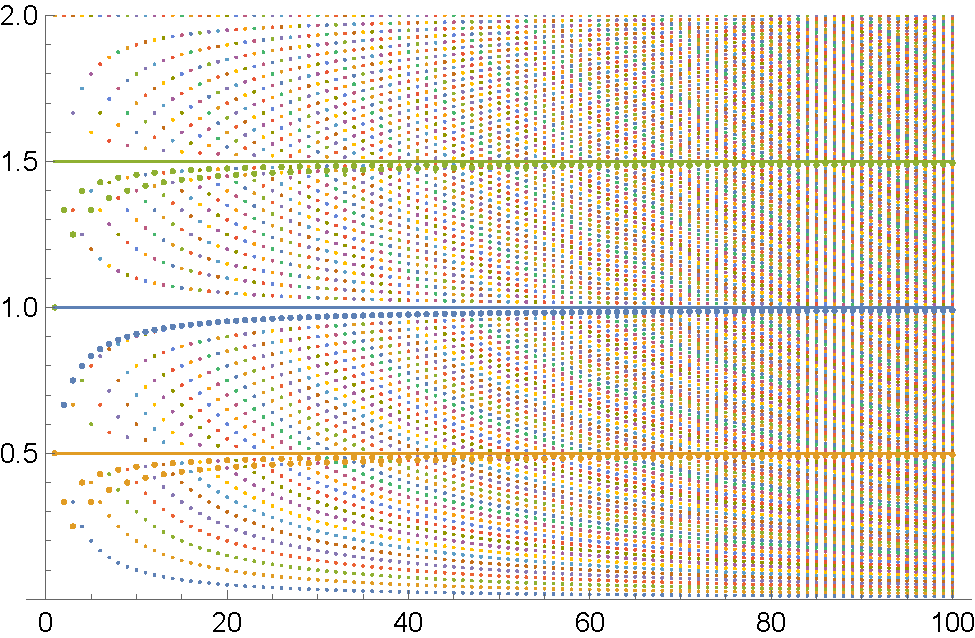
\includegraphics[width=0.5\textwidth]{../image/点列问题}
        \caption{\cref{例题1.2.1}第(3)问以$a_n=\frac{1}{n},b=0.5,1,1.5$为例}
    \end{figure}

    (3)对每个$a_i$,集合$Q_i=\{ka_i|k\in \mathbb{Z}\}$组成一个格点集:格点间距为$d_i=|a_i|$.

    对于每个实数$b$,总存在某个$k\in \mathbb{Z}$,使得$b\in[ka_i,(k+1)a_i]$,即$|b-ka_i|\le d_i$

    又$\lim\limits_{n\to \infty}a_n=0\Longrightarrow \forall \epsilon_m=\frac{1}{m}>0,\exists n_m$,有$0<|a_{n_m}|=d_{n_m}<\epsilon_m$

    对$b$和$a_{n_m}$,存在$k_m\in \mathbb{Z}$,使得$|b-k_ma_{n_m}|\le d_{n_m}<\epsilon_m$

    记$b_m=k_ma_{n_m}$,令$\epsilon_m\to 0$,即$m\to \infty$,则有$b_m\to b$,故$\{b_m\}\subset P$即为一个满足条件的数列
\end{proof}

\begin{example}
    证明:若$p_k>0(k=1,2,\cdots)$且$\lim\limits_{n\to \infty}\frac{p_n}{p_1+p_2+\cdots+p_n}=0$,$\lim\limits_{n \to \infty} a_n=a$,则$\lim\limits_{n\to \infty}\frac{p_1a_n+p_2a_{n-1}+\cdots+p_na_1}{p_1+p_2+\cdots+p_n}=a$
\end{example}

\begin{proof}

    欲解$|\frac{p_1a_n+p_2a_{n-1}+\cdots+p_na_1}{p_1+p_2+\cdots+p_n}-a|\le \frac{p_1|a_n-a|+\cdots+p_n|a_1-a|}{p_1+p_2+\cdots+p_n}<\epsilon$

    注意到$\lim\limits_{n\to \infty} a_n=a \Longrightarrow\forall \epsilon>0,\exists N_1 \in \mathbb{N}^+,\mbox{使得}n>N_1\mbox{时,有}|a_n-a|<\frac{\epsilon}{2}$,则
    $$\frac{p_1|a_n-a|+\cdots+p_{n-N_1}|a_{N_1+1}-a|+\cdots+p_n|a_1-a|}{p_1+p_2+\cdots+p_n}< \frac{\epsilon}{2}\cdot \frac{p_1+\cdots+p_{n-N_1}}{p_1+p_2+\cdots+p_n}+\frac{p_{n-N_1+1}|a_{N_1}-a|+\cdots+p_n|a_1-a|}{p_1+p_2+\cdots+p_n}$$
    $$<\frac{\epsilon}{2}+\frac{p_{n-N_1+1}|a_{N_1}-a|+\cdots+p_n|a_1-a|}{p_1+p_2+\cdots+p_n}$$

    设$M=\max \{|a_{N_1}-a|,\cdots,|a_1-a|\}$,
    则$\frac{p_{n-N_1+1}|a_{N_1}-a|+\cdots+p_n|a_1-a|}{p_1+p_2+\cdots+p_n}<\frac{p_{n-N_1+1}+\cdots+p_n}{p_1+p_2+\cdots+p_n}M$
    \begin{equation*}
        0<\frac{p_{n-i+1}}{p_1+p_2+\cdots+p_n}<\frac{p_{n-i+1}}{p_1+p_2+\cdots+p_{n-i+1}}\to 0\Longrightarrow \lim\limits_{n\to \infty}\frac{p_{n-i+1}}{p_1+p_2+\cdots+p_n}=0\quad i=2,\cdots,N_1
    \end{equation*}

    故$\lim\limits_{n\to \infty} \frac{p_{n-N_1+1}+\cdots+p_n}{p_1+p_2+\cdots+p_n} = 0
        \Longrightarrow
        \exists N_2\in \mathbb{N}^+$,使得$n>N_2$时,$\frac{p_{n-N_1+1}+\cdots+p_n}{p_1+p_2+\cdots+p_n}<\frac{\epsilon}{2M}$
    $$\forall \epsilon,\exists N=\max \{N_1,N_2\},\mbox{使得}n>N\mbox{时,有}|\frac{p_1a_n+p_2a_{n-1}+\cdots+p_na_1}{p_1+p_2+\cdots+p_n}-a|<\frac{\epsilon}{2}+\frac{\epsilon}{2M}\cdot M=\epsilon$$
    $$\Longrightarrow \lim\limits_{n\to \infty}\frac{p_1a_n+p_2a_{n-1}+\cdots+p_na_1}{p_1+p_2+\cdots+p_n}=a$$
\end{proof}

\begin{example}
    设实数列$\{x_n\}$满足$\lim\limits_{n\to \infty}(x_n-x_{n-2})=0$,证明:$\lim\limits_{n\to \infty}\frac{x_n-x_{n-1}}{n}=0$
\end{example}

\begin{proof}

    欲解$|\frac{x_n-x_{n-1}}{n}|<\epsilon$.

    设$y_n=|x_n-x_{n-1}|$,则$|x_n-x_{n-2}|=|x_n-x_{n-1}+x_{n-1}-x_{n-2}|\ge ||x_n-x_{n-1}|+|x_{n-1}-x_{n-2}||=|y_n-y_{n-1}|\ge 0$

    故$\lim\limits_{n\to \infty}|y_n-y_{n-1}|=0
        \Longrightarrow \forall \epsilon>0,\exists N_1\in \mathbb{N}^+,\mbox{使得}n>N_1\mbox{时},|y_n-y_{n-1}|<\epsilon$

    则$$|\frac{x_n-x_{n-1}}{n}|=\frac{y_n}{n}\le
        \frac{|y_n-y_{n-1}|+|y_{n-1}-y_{n-2}|+\cdots +|y_{N_1+1}-y_{N_1}|}{n}+\frac{y_{N_1}}{n}<\frac{(n-N_1)}{n}\cdot \frac{\epsilon}{2}+\frac{y_{N_1}}{n}<\frac{\epsilon}{2}+\frac{y_{N_1}}{n}$$

    又$\exists N_2\in \mathbb{N}^+$,使得$n>N_2$时,有$\frac{y_{N_1}}{n}<\frac{\epsilon}{2}$

    故$\forall \epsilon,\exists N=\max \{N_1,N_2\}$,使得$n>N$时,有$|\frac{x_n-x_{n-1}}{n}|<\frac{\epsilon}{2}+\frac{\epsilon}{2}=\epsilon\Longrightarrow \lim\limits_{n\to \infty}\frac{x_n-x_{n-1}}{n}=0$
\end{proof}

\begin{definition}[函数极限$\epsilon-\delta$语言]
    \begin{equation*}
        \forall \epsilon>0,\exists \delta>0,\mbox{使得}0<|x-x_0|<\delta\mbox{时,有}|f(x)-a|<\epsilon\Longleftrightarrow \lim\limits_{x\to x_0} f(x)=a
    \end{equation*}
\end{definition}

\begin{example}
    按极限定义($\epsilon-\delta$语言)证明:$\lim\limits_{x\to 1}\sqrt{\frac{7}{16x^2-9}}=1$
\end{example}

\begin{proof}
    欲解$|\sqrt{\frac{7}{16x^2-9}}-1|<\epsilon$得$|x-1|<\delta(\epsilon)$.考虑放缩.
    $$|\sqrt{\frac{7}{16x^2-9}}-1|=|\frac{\frac{7}{16x^2-9}-1}{\sqrt{\frac{7}{16x^2-9}}+1}|\le |\frac{7}{16x^2-9}-1|=\frac{16|x+1||x-1|}{|(4x+3)(4x-3)|}\le \frac{16|x+1||x-1|}{3|4x-3|}$$

    还是较难. 考虑分步法,设$|x-1|<1$,则$0<x<2\Longrightarrow |x+1|<3\Longrightarrow \frac{16|x+1||x-1|}{3|4x-3|}<\frac{16|x-1|}{|4x-3|}=\frac{4|x-1|}{|x-\frac{3}{4}|}$

    进一步,设$|x-1|<\frac{1}{8}$,则$\frac{7}{8}<x<\frac{9}{8}\Longrightarrow |x-\frac{3}{4}|>\frac{1}{8}\Longrightarrow \frac{16|x+1||x-1|}{3|4x-3|}<32|x-1|$
    $$\forall \epsilon>0,\exists \delta=\min \{\frac{1}{8},\frac{1}{32}\epsilon\},\mbox{使得}0<|x-1|<\delta\mbox{时,有}|\sqrt{\frac{7}{16x^2-9}}-1|<\epsilon\Longrightarrow \lim\limits_{x\to 1}\sqrt{\frac{7}{16x^2-9}}=1$$
\end{proof}

\subsubsection{拟合法}

\begin{note}
    为了证明$\lim \limits_{n \to \infty}x_n=A$,关键在于证明$|x_n-A|$能够任意小. 为此,一般尽可能将$x_n$化简.值得注意的是,有时候$x_n$难以化简,反而$A$能够“化繁”,写成与$x_n$类似的形式.这种方法称为“拟合法”.“拟合法”思想的实质,是将单位“1”进行适当的分解.
\end{note}

\vspace{8pt}
\begin{example}\label{例题1.2.5}
    设$x\to 0$时,$f(x)\thicksim x,x_n=\sum\limits_{i=1}^{n}f(\frac{2i-1}{n^2}a)$,试证明$\lim \limits_{n \to \infty}x_n=a(a>0)$
\end{example}

\begin{proof}
    注意到$a=\sum\limits_{i=1}^{n}\frac{2i-1}{n^2}a$,从而有$
        |x_n-a|
        =|\sum\limits_{i=1}^{n}f(\frac{2i-1}{n^2}a)-\sum\limits_{i=1}^{n}\frac{2i-1}{n^2}a|
        =\sum\limits_{i=1}^{n}|f(\frac{2i-1}{n^2}a)-\frac{2i-1}{n^2}a|$

    若能证明$\forall \epsilon>0$时,
    \begin{equation}\label{式1.2.1}
        \exists N\in \mathbb{N}^+,\mbox{使得}n>N\mbox{时},|f(\frac{2i-1}{n^2}a)-\frac{2i-1}{n^2}a|<\frac{2i-1}{n^2}\epsilon\quad i=1,2,\cdots,n
    \end{equation},

    则有$n>N$时,
    $|x_n-a|
        =\sum\limits_{i=1}^{n}|f(\frac{2i-1}{n^2}a)-\frac{2i-1}{n^2}a|
        <\sum\limits_{i=1}^{n}\frac{2i-1}{n^2} \epsilon=\epsilon
    $,即$\lim \limits_{n \to \infty}x_n=a(a>0)$得证

    欲证\cref{式1.2.1},即证$$\exists N\in \mathbb{N}^+,\mbox{使得}n>N\mbox{时},|\frac{f(\frac{2i-1}{n^2}a)}{\frac{2i-1}{n^2}a}-1|<\frac{\epsilon}{a}\quad i=1,2,\cdots,n$$

    事实上,由于$x\to 0\mbox{时},f(x)\thicksim x \Longrightarrow \forall \epsilon,\exists \delta>0,0<|x|<\delta$时,$|\frac{f(x)}{x}-1|<\frac{\epsilon}{a}$

    令$\frac{2i-1}{n^2}a
        <\frac{2n-1}{n^2}a
        <\frac{2n}{n^2}a
        =\frac{2}{n^2}a<\frac{2a}{n}
        <\delta$
    解得$n>\frac{2a}{\delta}$,令$N=[\frac{2a}{\delta}]+1$,

    则$n>N\mbox{时},0<\frac{2i-1}{n^2}a<\delta\Longrightarrow|\frac{f(\frac{2i-1}{n^2}a)}{\frac{2i-1}{n^2}a}-1|<\frac{\epsilon}{a}$.得证
\end{proof}

\begin{practice}
    证明:

    (1)$\lim \limits_{n \to \infty} \prod \limits_{i=1}^{n} (1+\frac{2i-1}{n^2}a^2)=e^{a^2}$\quad
    (2)$\lim \limits_{n \to \infty}  \prod \limits_{i=1}^{n+1} \cos \frac{\sqrt{2i-1}}{n}a^2=e^{-\frac{a^4}{2}}$
\end{practice}

\begin{proof}
    (1)两边取对数,得需证
    $\lim \limits_{n \to \infty} \sum \limits_{i=1}^{n} \ln(1+\frac{2i-1}{n^2}a^2)=a^2$

    $x\to 0$时,$f(x)=\ln (1+x) \thicksim x $,则由\cref{例题1.2.5}得,$\lim \limits_{n \to \infty} \sum \limits_{i=1}^{n} \ln(1+\frac{2i-1}{n^2}a^2)
        =\lim \limits_{n \to \infty} \sum \limits_{i=1}^{n} f(\frac{2i-1}{n^2}a^2)
        =a^2$

    (2)两边取对数,得需证
    $\lim \limits_{n \to \infty} \sum \limits_{i=1}^{n+1} \ln(\cos \frac{\sqrt{2i-1}}{n}a^2)=-\frac{a^4}{2}$

    $x\to 0$时,$f(x)=\ln \cos x=\ln [1+(\cos x-1)] \thicksim (\cos x-1) \thicksim -2\sin^2 \frac{x}{2} \thicksim -\frac{x^2}{2}$

    同\cref{例题1.2.5}考虑拟合法,可证$\lim \limits_{n \to \infty} \sum \limits_{i=1}^{n} \ln(1+\frac{2i-1}{n^2}a^2)
        =\lim \limits_{n \to \infty} \sum \limits_{i=1}^{n} f(\frac{\sqrt{2i-1}}{n}a^2)
        =-\frac{(a^2)^2}{2}
        =-\frac{a^4}{2}$
\end{proof}

\begin{practice}\label{小试牛刀1.2.2}
    设$\lim \limits_{n \to \infty} a_n = a$,试证:
    \begin{equation*}
        \lim \limits_{n \to \infty} \frac{1}{2^n} (a_0+C_n^1 a_1 + C_n^2 a_2 + \cdots + C_n^k a_k + \cdots + a_n)=a
    \end{equation*}
\end{practice}

\begin{proof}
    $a = \frac{2^n}{2^n} a
        =\frac{\sum\limits_{k=0}^{n} C_n^k}{2^n} a
        =\frac{1}{2^n} \sum\limits_{k=0}^{n} C_n^k a \Longrightarrow |\frac{1}{2^n} \sum\limits_{k=0}^{n} C_n^k a_k - a|
        =|\frac{1}{2^n} \sum\limits_{k=0}^{n} C_n^k a_k - \frac{1}{2^n} \sum\limits_{k=0}^{n} C_n^k a|
        \le \frac{1}{2^n} \sum\limits_{i=0}^{n} C_n^k |a_k-a|$

    又$\lim \limits_{n \to \infty} a_n = a
        \Longrightarrow \forall \epsilon>0,\exists k_0 \in \mathbb{N}^+,\mbox{使得}k>k_0时,|a_k-a|<\frac{\epsilon}{2}$

    而$k<k_0$时,记$M=\max |a_k-a|$,则$|a_k-a|\le M$

    故$\frac{1}{2^n} \sum\limits_{k=0}^{n} C_n^k |a_k-a|=\frac{1}{2^n} \sum\limits_{k=0}^{k_0-1} C_n^k |a_k-a| + \frac{1}{2^n} \sum\limits_{k=k_0}^{n} C_n^k |a_k-a|< \frac{Mk_0n^{k_0}}{2^n} + \frac{\epsilon}{2}$

    又$\lim \limits_{n \to \infty} \frac{Mk_0n^{k_0}}{2^n}=0 \Longrightarrow \exists N>k_0>0$,使得$n>N$时,有$|\frac{1}{2^n} \sum\limits_{k=0}^{n} C_n^k a_k - a| < \frac{Mk_0n^{k_0}}{2^n} + \frac{\epsilon}{2}<\frac{\epsilon}{2} + \frac{\epsilon}{2}<\epsilon$

    即$\lim \limits_{n \to \infty} \frac{1}{2^n} (a_0+C_n^1 a_1 + C_n^2 a_2 + \cdots + C_n^k a_k + \cdots + a_n)=a$得证
\end{proof}

\begin{practice}
    若\cref{小试牛刀1.2.2}中$\frac{C_n^k}{2^n}$改为一般的实数$\alpha_{n,k},\forall n\in \mathbb{N}:k=0,1,\cdots,n$,问$a_{n,k}$应该满足什么条件,该命题依然成立?即当$\lim \limits_{n \to \infty}a_n=a\Longrightarrow \lim \limits_{n \to \infty} \sum\limits_{k=0}^{n} \alpha_{n,k}a_k=a$
\end{practice}

\begin{solution}
    $\sum\limits_{k=1}^{n} a_{n,k}=1$
\end{solution}

\subsubsection{用邻域描述极限}
\begin{definition}[邻域]
    区间$(a-\epsilon,a+\epsilon)$称为点$a$的$\epsilon-$领域,用$U(a,\epsilon)$表示。

    区间$(a-\epsilon,a)\bigcup (a,a+\epsilon)$称为$a$的$\epsilon-$去心邻域,用$\overset{\circ}{U}(a,\epsilon)$表示。
\end{definition}

\begin{note}
    
    使用邻域语言,可以将定义\ref{数列极限}中的$\epsilon-\delta$语言表述为以下的等价形式

    \begin{enumerate}
        \item $\lim \limits_{n \to \infty} a_n = a \Longleftrightarrow \forall \epsilon>0, \exists N\in \mathbb{N}^+,\mbox{使得}\forall n>N\mbox{时},\mbox{有} a_n\in U(a,\epsilon)$
        \item $\lim \limits_{n \to \infty} a_n = a \Longleftrightarrow \forall \epsilon>0, \mbox{只有有限个}n\in \mathbb{N^+},\mbox{使得}a_n\notin U(a,\epsilon)$
        \item $\lim \limits_{n \to \infty} a_n = a \Longleftrightarrow \forall \epsilon>0,U(a,\epsilon)$之外仅有$a_n$的有限项
    \end{enumerate}
\end{note}

\vspace{3pt}
\begin{example}
    设$f:\mathbb{N} \rightarrow \mathbb{N}_1$,$n=f(m)$($\mathbb{N}$和$\mathbb{N}_1$都是全体自然数组成的空间),且$\forall n\in \mathbb{N}:f^{-1}(n)$为有限集.试证明:若$\lim \limits_{n \to \infty} a_n =a$,则$\lim \limits_{m \to \infty} a_{f_{(m)}}=a$
\end{example}

\begin{proof}

    [法1]$\lim \limits_{n \to \infty} a_n = a \Longleftrightarrow \forall \epsilon>0,U(a,\epsilon)$之外仅有$a_n$的有限项

    把这$U(a,\epsilon)$之外的有限项记作$\{a_{n_j}\}_{j=1}^k={a_{}}=\{a_{n_1},a_{n_2},\cdots,a_{n_k}\}$

    又根据题意得,$f^{-1}(n_j)=\{m|n_j=f_m\}$为有限集,它们的并$E=\underset{j=1}{\overset{k}{\bigcup}} \{m|n_j=f(m)\}$仍然是有限集。

    故$\forall \epsilon>0,U(a,\epsilon)$之外仅有$a_{f_{(m)}}$的有限项:$\{a_{f_{(m)}|m\in E}\} \Longleftrightarrow \lim \limits_{m \to \infty} a_{f_{(m)}}=a$

    [法2]$\lim \limits_{n \to \infty} a_n = a \Longleftrightarrow \forall \epsilon>0, \exists N\in \mathbb{N}^+,\mbox{使得}\forall n>N\mbox{时},\mbox{有} a_n\in U(a,\epsilon)$

    又根据题意得,$\forall n\in \mathbb{N}:f^{-1}(n)$为有限集,则$\underset{n\le N}{\bigcup} f^{-1}(n)$为有限集,$\exists M=\max \underset{n\le N}{\bigcup} f^{-1}(n)$,

    则$m>M$时,有$a_m\in U(a,\epsilon) \Longrightarrow \lim \limits_{m \to \infty} a_{f_{(m)}}=a$

    [法3]只需证明$\{f(m)\}_{m=1}^{\infty}$是$\{n\}_{n=1}^{\infty}$的子列(不需要单调增,只需要趋于$+\infty$即可),则根据数列与子列关系,
    
    有$\lim \limits_{n \to \infty} a_n=a \Longrightarrow \lim \limits_{m \to \infty} a_{f_{(m)}}=a$

    事实上,若$\{f(m)\}_{m=1}^{\infty}$是$\{n\}_{n=1}^{\infty}$的子列,则说明$\{f(m)\}_{m=1}^{\infty}$只是$\{n\}_{n=1}^{\infty}$中的有限项,也就是说:$\{n\}_{n=1}^{\infty}$中的有限项对应着$\{f(m)\}_{m=1}^{\infty}$中的无穷多项。

    因此,至少存在一个$n$通过$n=f(m)$对应着无穷多个$m$。这与题设“$\forall n\in \mathbb{N}:f^{-1}(n)$为有限集”矛盾
\end{proof}

\subsection{用柯西收敛准则证明极限}
\begin{theorem}[柯西(Cauchy)收敛准则]
    数列$\{x_n\}$收敛 
    
    $\Longleftrightarrow \forall \epsilon>0,\exists N\in \mathbb{N}^+$,使得$\forall m,n>N$,有$|x_m-x_n|<\epsilon$

    $\Longleftrightarrow \forall \epsilon>0,\exists N\in \mathbb{N}^+$,使得$n>N\mbox{时},\forall p\in \mathbb{N}^+$,有$|x_{n+p}-x_n|<\epsilon$
\end{theorem}

\begin{example}
    设$\displaystyle x_n=\frac{\sin 1}{2}+\frac{\sin 2}{2^2}+\cdots+\frac{\sin n}{2^n}$,试证$\{x_n\}$收敛
\end{example}

\begin{proof}
    $$|x_{n+p}-x_n|
    =|\frac{\sin (n+1)}{2^{n+1}}+\cdots+\frac{\sin (n+p)}{2^{n+p}}|
    \le |\frac{\sin (n+1)}{2^{n+1}}|+\cdots+|\frac{\sin (n+p)}{2^{n+p}}|
    \le \frac{1}{2^{n+1}}+\cdots+\frac{1}{2^{n+p}}$$
    $$=\frac{1}{2^{n+1}} \cdot \frac{1-\frac{1}{2^p}}{1-\frac{1}{2}}
    <\frac{1}{2^n}<\frac{1}{n}$$

    解$|x_{n+p}-x_n|<\frac{1}{n}<\epsilon$得$n>\frac{1}{\epsilon}$

    因此,$\forall \epsilon>0,\exists N=[\frac{1}{\epsilon}]+1\in \mathbb{N}^+$,使得$n>N$时,$\forall p\in \mathbb{N}^+$,有$|x_{n+p}-x_n|<\epsilon$

    由柯西收敛准则得,数列$\{x_n\}$收敛 
\end{proof}

\clearpage
\begin{example}
    判断以下命题的真伪:

    数列$\{a_n\}$存在极限$\lim \limits_{n \to \infty} a_n =a$的充分必要条件是:对任意$p\in \mathbb{N}^+$,都有$\lim \limits_{n \to \infty}|a_{n+p}-a_n|=0$
\end{example}

\begin{solution}
    
    该命题不对.如$a_n=\sqrt{n}$,虽然$\lim \limits_{n \to \infty}|a_{n+p}-a_n|
    =\lim \limits_{n \to \infty}|\sqrt{n+p}-\sqrt{n}|
    =\lim \limits_{n \to \infty} \frac{p}{\sqrt{n+p}+\sqrt{n}}
    =0$

    但$\lim \limits_{n \to \infty} a_n =+\infty$,即数列$\{a_n\}$不存在极限
\end{solution}

\subsection{否定形式及 \texorpdfstring{$\forall$}{} 和 \texorpdfstring{$\exists$}{} 的使用法则}

\begin{theorem}[数列不收敛]
    数列$\{x_n\}$不收敛

    $\Longleftrightarrow \forall A \in \mathbb{R}, \exists \epsilon_0 > 0,\forall N\in \mathbb{N}^+,\exists n_0 > N$,使得$|x_{n_0}-A|\ge \epsilon_0$ \qquad (极限定义的否定形式)
    
    $\Longleftrightarrow \exists \epsilon_0 > 0,\forall N\in \mathbb{N}^+,\exists m_0,n_0 > N$,使得$|x_{m_0}-x_{n_0}|\ge \epsilon_0 $ \qquad (柯西收敛准则的否定形式1)

    $\Longleftrightarrow \exists \epsilon_0 > 0,\forall N\in \mathbb{N}^+,\exists n_0>N,p_0\in \mathbb{N}^+$,使得$|x_{n_0+p_0}-x_{n_0}|\ge \epsilon_0 $\qquad (柯西收敛准则的否定形式2)
\end{theorem}

\begin{example}
    证明:$\lim \limits_{n \to \infty} \sin n$不存在
\end{example}

\begin{proof}
    
    [法1]根据极限定义的否定形式,我们需证明:$ \forall A \in \mathbb{R}, \exists \epsilon_0 > 0,\forall N\in \mathbb{N}^+,\exists n_0 > N$,使得$|x_{n_0}-A|\ge \epsilon_0$

    当$|A|>1$时,$\forall n\in \mathbb{N}^+,|\sin n - A| \ge ||\sin n|-|A||=|A|-|\sin n|\ge |A|-1>0$

    当$0\le A \le 1$时,$\forall N\in \mathbb{N}^+,\exists n_0=[(2N\pi - \frac{\pi}{2})+\frac{\pi}{4}]>N$,
    
    有$2N\pi - \frac{\pi}{2}-\frac{\pi}{4} < n_0 < 2N\pi -\frac{\pi}{2}+\frac{\pi}{4} \Longrightarrow -1 < \sin n_0 < -\frac{\sqrt{2}}{2}$,
    则$|\sin n_0 -A|=A-\sin n_0 > A+\frac{\sqrt{2}}{2}\ge \frac{\sqrt{2}}{2}$

    当$-1\le A<0$时,$\forall N\in \mathbb{N}^+,\exists n_0=[(2N\pi + \frac{\pi}{2})+\frac{\pi}{4}]>N$,
    
    有$2N\pi + \frac{\pi}{2}-\frac{\pi}{4} < n_0 < 2N\pi +\frac{\pi}{2}+\frac{\pi}{4} \Longrightarrow \frac{\sqrt{2}}{2} < \sin n_0 < 1 $,
    则$|\sin n_0 -A|=\sin n_0 - A > \frac{\sqrt{2}}{2} - A \ge \frac{\sqrt{2}}{2}$

    [法2]根据柯西收敛准则的否定形式1,我们需证明$\exists \epsilon_0 > 0,\forall N\in \mathbb{N}^+,\exists m_0,n_0 > N$,使得$|x_{m_0}-x_{n_0}|\ge \epsilon_0 $

    事实上,取$\epsilon_0=\frac{\sqrt{2}}{2},m_0=[2N\pi + 2\pi] ,n_0=[2N\pi + \frac{3\pi}{4}]$

    有$m_0,n_0>N$,且$2N\pi + \pi <m_0< 2N\pi + 2\pi,2N\pi +\frac{\pi}{4}<n_0<2N\pi + \frac{3\pi}{4}\Longrightarrow -1<\sin m_0<0,\frac{\sqrt{2}}{2}<\sin n_0<1$,
    
    则$|\sin m_0-\sin n_0|=\sin n_0-\sin m_0>\frac{\sqrt{2}}{2}=\epsilon_0$

    [法3]用反证法。假设$\lim \limits_{n \to \infty} \sin n=A$.
    
    由$\sin(n+2)-\sin n=\sin(n+1+1)-\sin (n+1-1)=2sin 1 \cos (n+1)$得
    
    $\lim \limits_{n \to \infty} \cos (n+1)=\lim \limits_{n \to \infty} [\sin(n+2)-\sin n]=A-A=0$,即$\lim \limits_{n \to \infty} \cos n = 0$

    则$A=\lim \limits_{n \to \infty} \sin n = \lim \limits_{n \to \infty} \sqrt{1-\cos^2 n} = 1$

    又$A=\lim \limits_{n \to \infty} \sin 2n=\lim \limits_{n \to \infty} 2\cos n \sin n = 0$

    所以产生矛盾。$\lim \limits_{n \to \infty} \sin n$不存在
\end{proof}







\end{document}